\documentclass{article}
\usepackage{graphicx} % Required for inserting images
\usepackage[utf8]{inputenc}
\usepackage[russian]{babel}
\usepackage[left=1.5cm, right=2cm, top=1cm, bottom=2cm]{geometry}


\begin{document}

\begin{titlepage}
	\begin{center}
		{\large МОСКОВСКИЙ ФИЗИКО-ТЕХНИЧЕСКИЙ ИНСТИТУТ (НАЦИОНАЛЬНЫЙ ИССЛЕДОВАТЕЛЬСКИЙ УНИВЕРСИТЕТ)}
	\end{center}
	\begin{center}
		{\large Физтех-школа фотоники, электроники и молекулярной физики}
	\end{center}


	\vspace{4.5cm}
	{\huge
		\begin{center}
			{\bf Лабораторная работа }\\
			Исследование длиннобазового лазерного интерферометра
		\end{center}
	}
	\vspace{2cm}
	\begin{flushright}
		{\LARGE Авторы:\\
			Доля Артем\\
			Кулагин Никита\\
			Шмаков Владимир \\
			\vspace{0.2cm}
			Б04-105}
	\end{flushright}
	\vspace{8cm}
	\begin{center}
		Долгопрудный 2024
	\end{center}
\end{titlepage}


\newpage
\section{Цель работы}
\begin{itemize}
	\item Найти зависимость видности от времени работы лазера
	\item Найти зависимость видности от разности хода
\end{itemize}
\section{Экспериментальная установка}
\begin{figure}[htp]
	\centering
	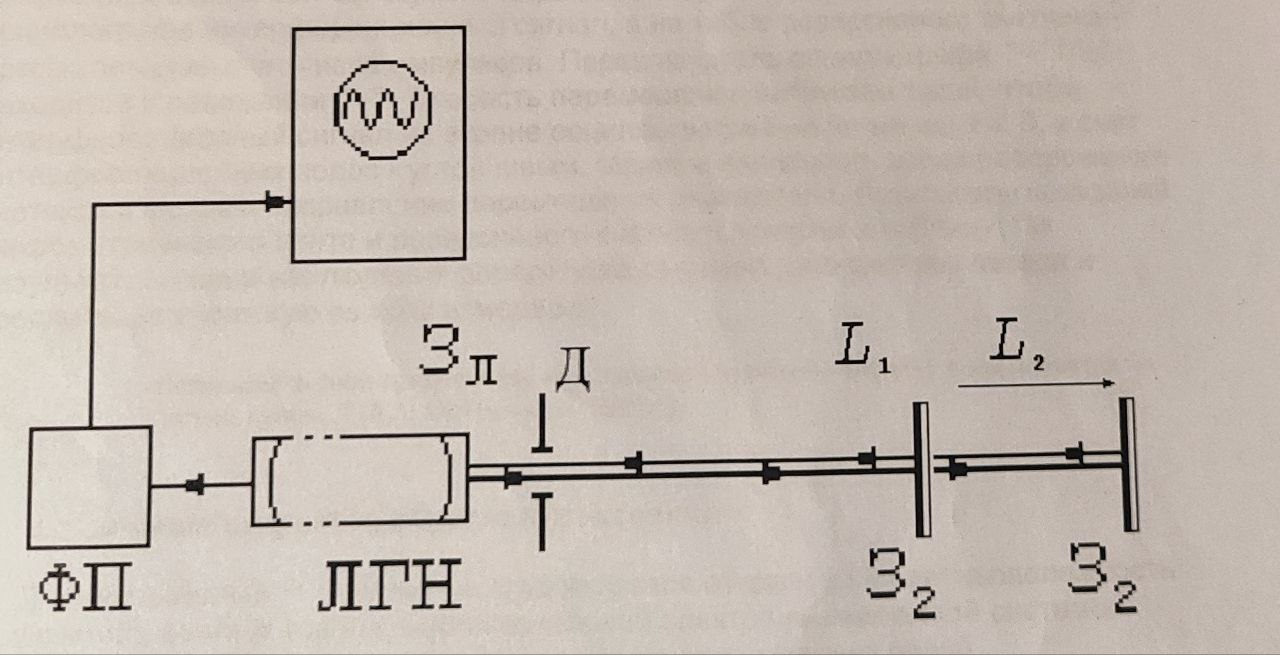
\includegraphics[width=0.5\textwidth]{megahuinya.jpg}
	\caption{Установка}
	\label{pic:experimental_setup}
\end{figure}

Экспериментальная установка состоит их лазерного генератора(ЛГН).
И двух зеркал, расстояние между которыми $L_{2}$ фиксировано.

Для наблюдения интерференционной картины используется фотоприёмник и
осциллограф.

\section{Ход работы}
Мы собрали схему на рис. 1. и измеряли изменение амплитуды интерференционного сигнала при расположении зеркала \(3_2\) на разных расстояниях от лазера.
На основе полученных данных рассчитывали видность картины. Данные приведены ниже
\begin{figure}[htp]
	\centering
	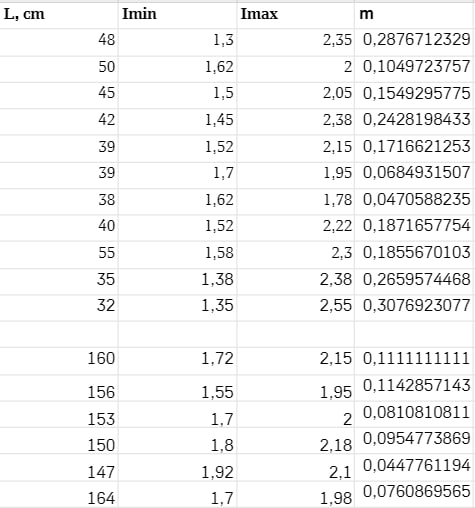
\includegraphics[width=0.5\textwidth]{dermo.jpg}
	\caption{Экспериментальные данные}
	\label{pic:experimental_data}
\end{figure}
\section{Обработка результатов эксперимента}

\subsection{Эксперимент 1}

Экспериментальная зависимость видности от расстояния между лазером и зеркалами
изображена на рисунке ниже
\begin{figure}[htbp]
	\centering
	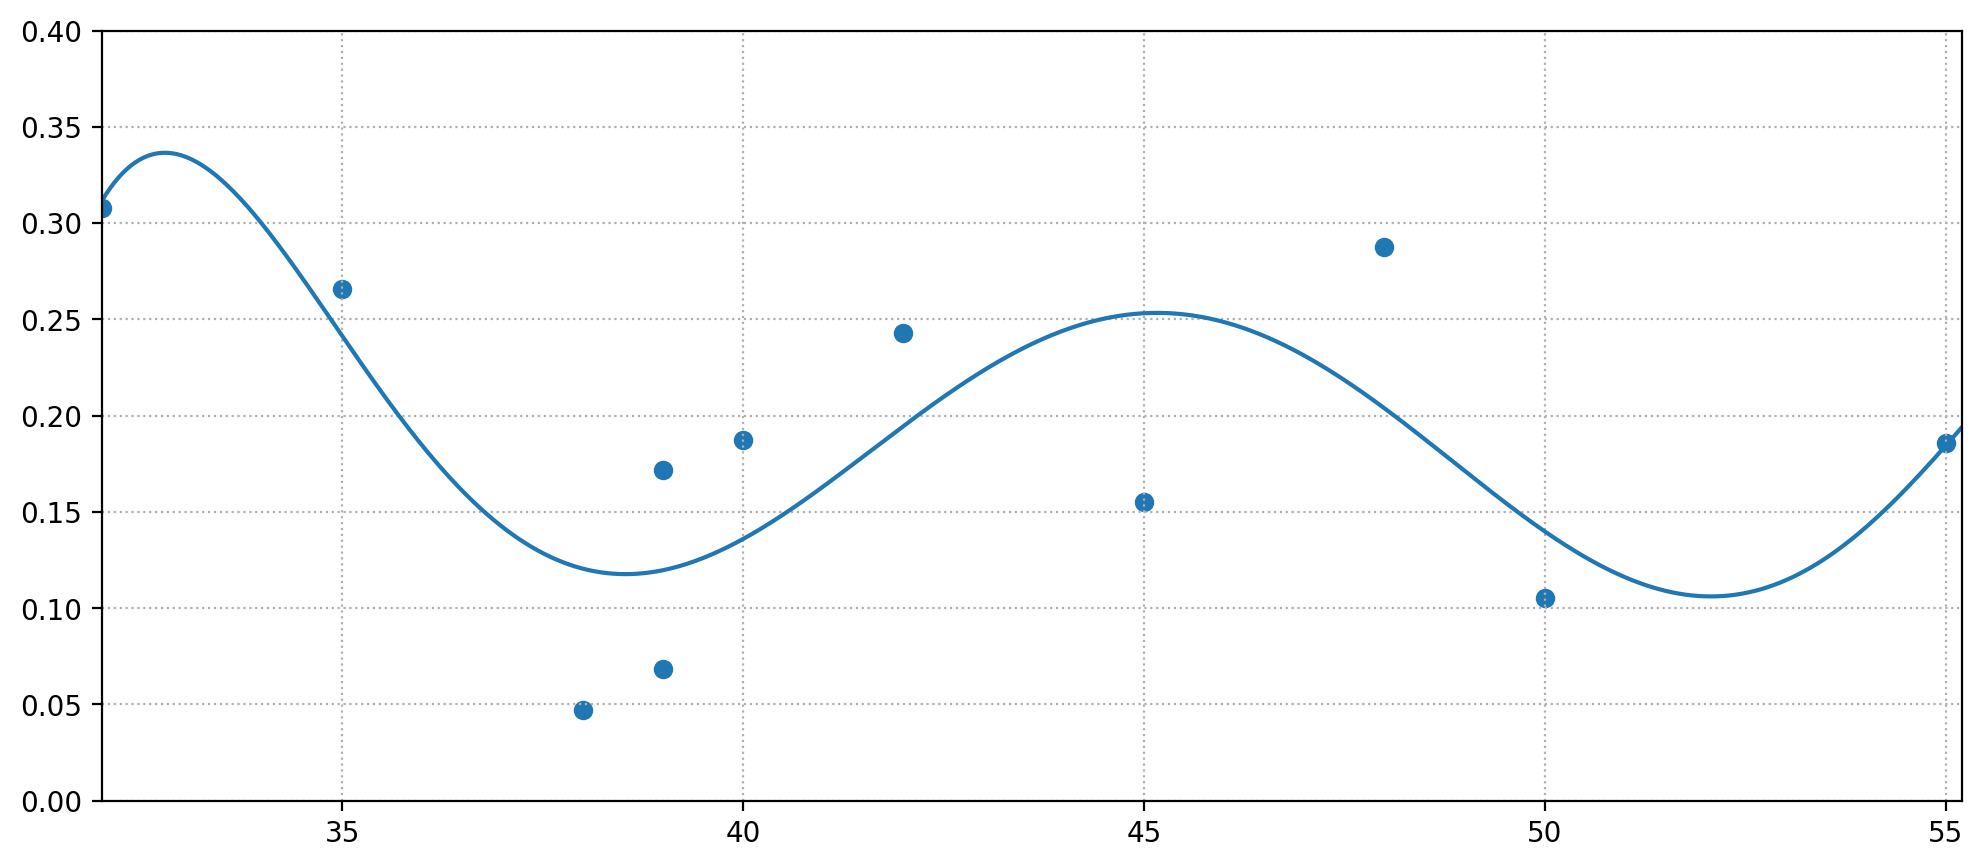
\includegraphics[width = 0.7 \textwidth]{data_1.png}
	\caption{Результаты первого эксперимента(грубое приближение полиномом пятой степени)}
	\label{pic:exp_1}
\end{figure}

Отодвинем зеркало на достаточно большое расстояние $L_{1} >> L_{2}$.
\begin{figure}[htbp]
	\centering
	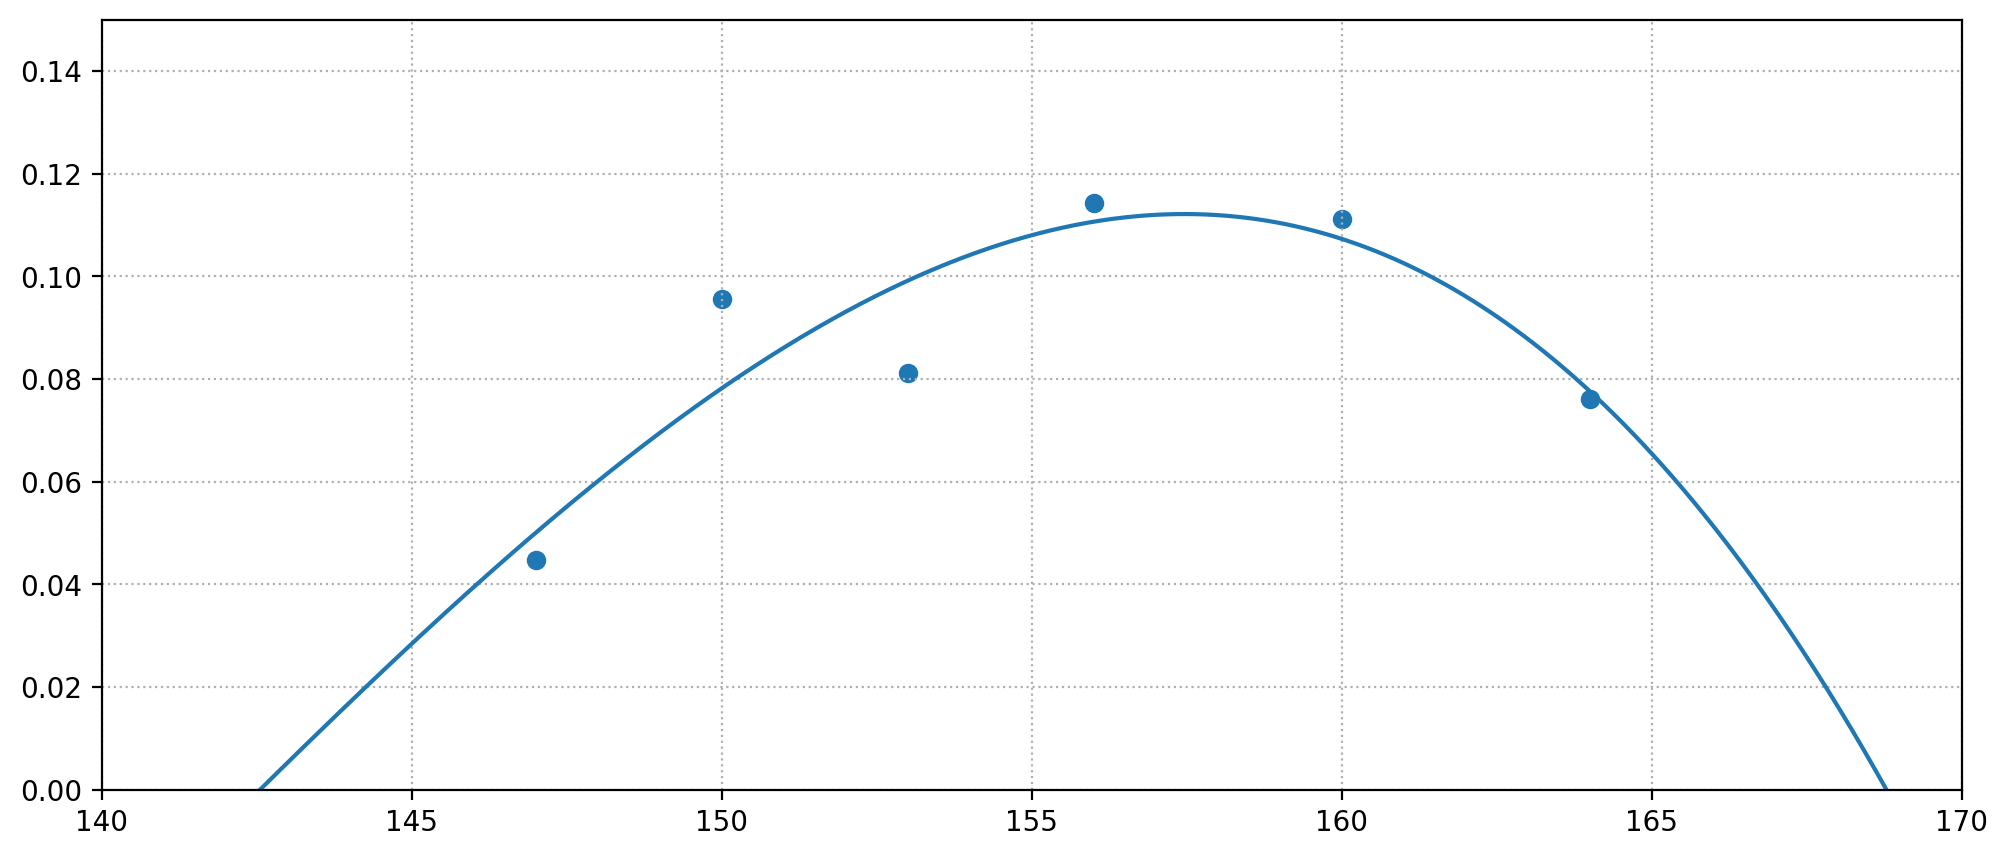
\includegraphics[width = 0.7 \textwidth]{data_2.png}
	\caption{Зависимость видности от расстояния между лазером и зеркалами}
	\label{pic:exp_2}
\end{figure}


\subsection{Эксперимент 2}

Зависимости видности от времени при $L = 16 \text{ см}$ и $L = 24 \text{ см}$ изображены
на рисунках ниже. На обеих фигурах видно, что в с ростом времени возрастает
среднее значение видности.
\begin{figure}[htbp]
	\centering
	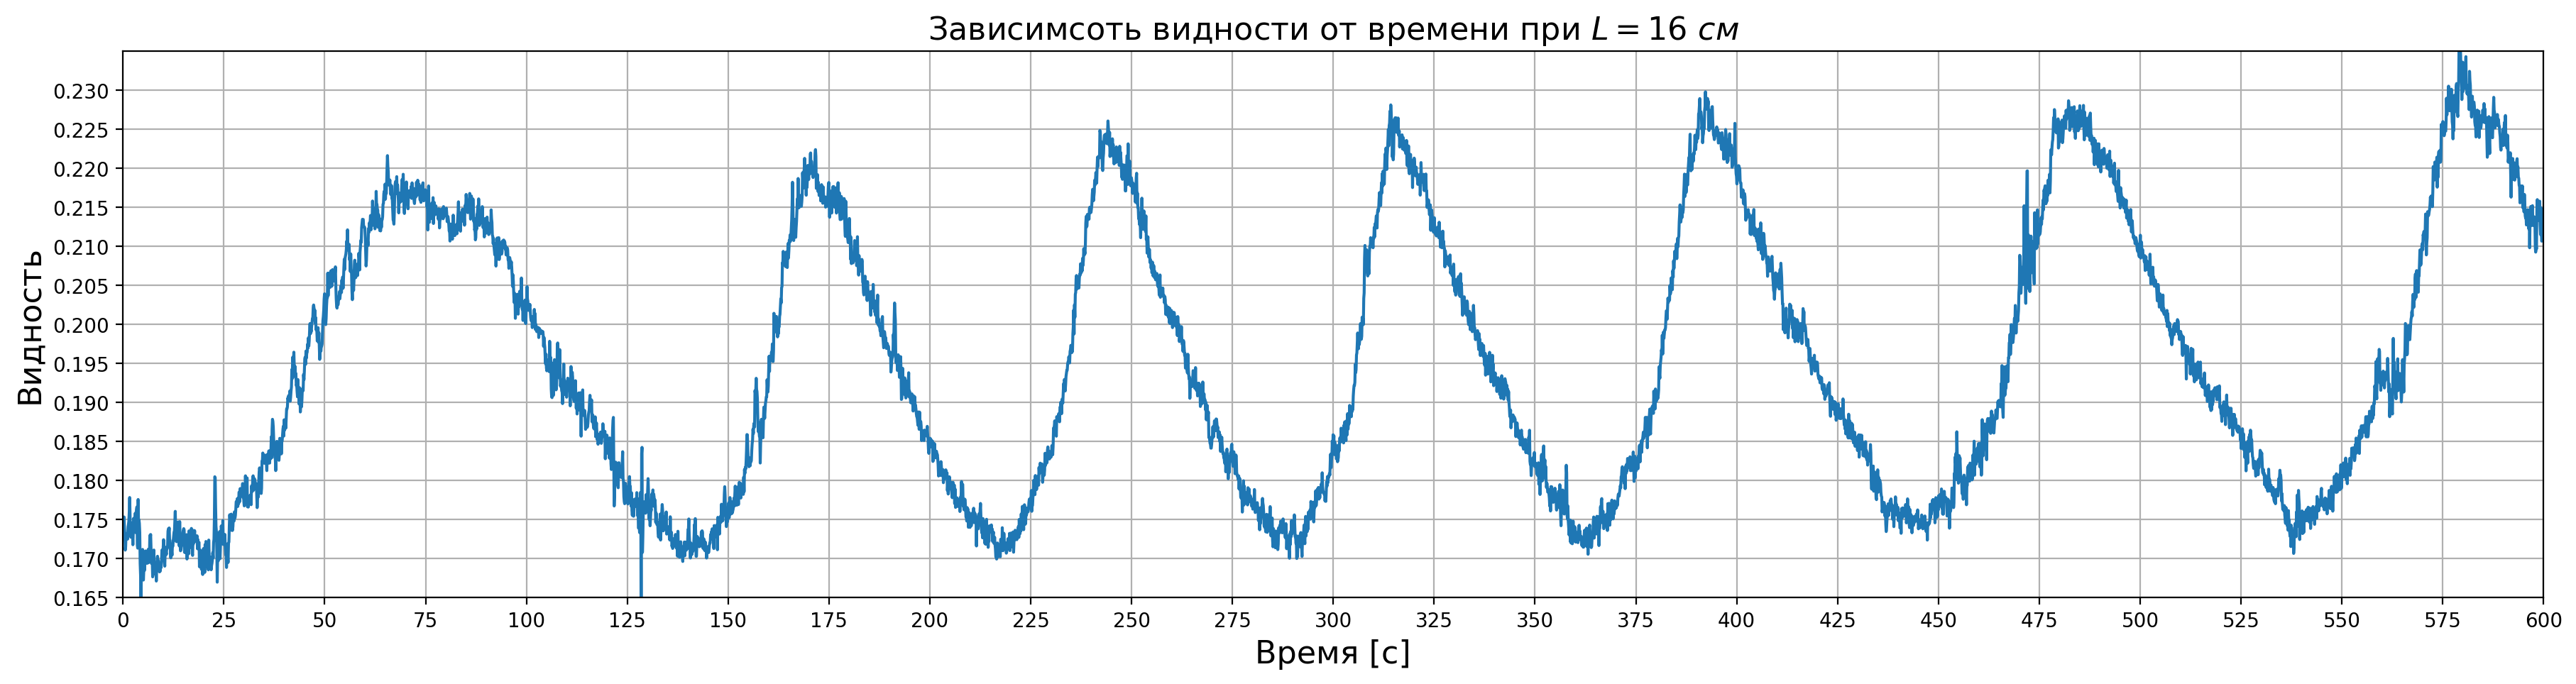
\includegraphics[width = 1\textwidth]{L_16cm.png}
	\caption{Зависимость видности от времени при L = 16 см}
	\label{pic:L_16}
\end{figure}

\begin{figure}[htbp]
	\centering
	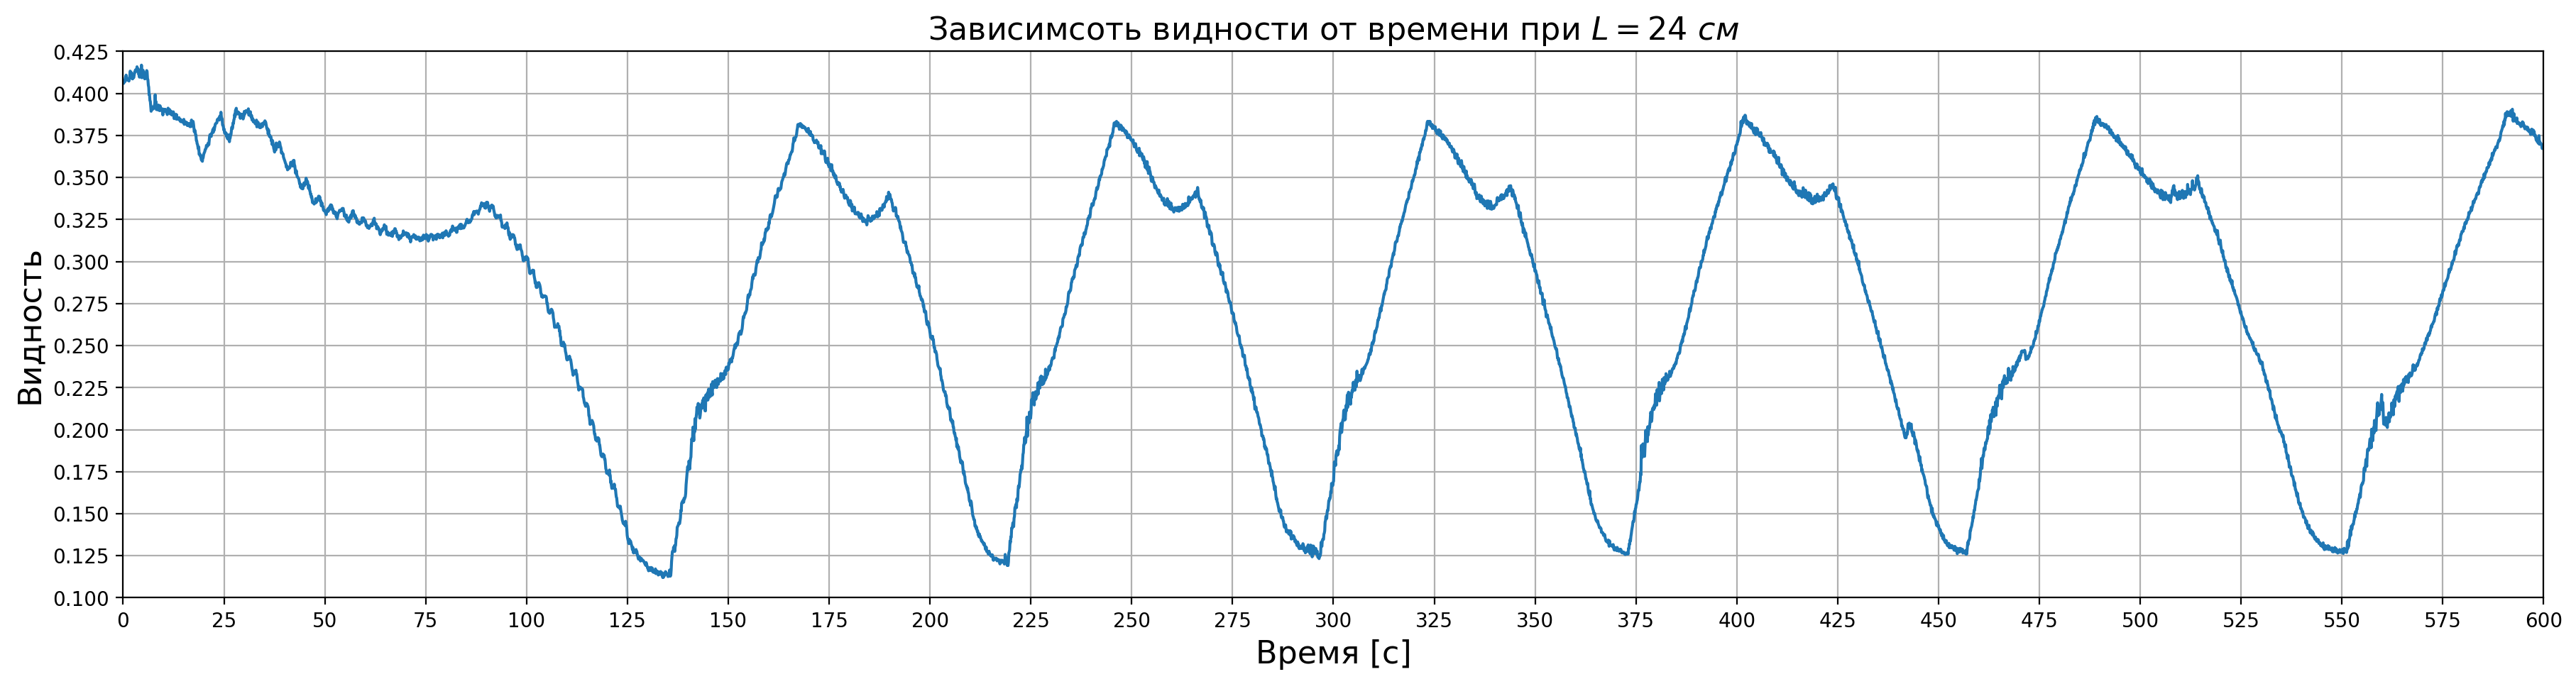
\includegraphics[width = 1 \textwidth]{L_24cm.png}
	\caption{Зависимость видности от времени при L = 24см}
	\label{pic:L_24}
\end{figure}


\newpage

\section{Вывод}

\begin{itemize}
	\item Получены зависимости видности интерференционной картины от расстояния между генератором и зеркалами.
	      При этом зависимость при большом $L$ похожа на зависимость при малом $L$.
	\item Во втором эксперименте были получены зависимости видности интерференционной
	      картины от времени. Видно, что среднее значение видности растет.

\end{itemize}
\end{document}